\subsection{Slant Incident HWP properties}

\paragraph{Description:}
At non-normal incidence, the HWP optical properties change. This effect is small for angles $<$10 degrees away from the normal incidence and increases for larger angular deviations. Stray light, emissions, and reflections in the instrument can produce off-axis radiation crossing the HWP.

\textbf{What systematics do these contribute to?}

\subsubsection{Birefringent HWP}

\paragraph{Plan to model and/or measure:}
For a birefringent HWP, how the optical properties change with the incidence angle can be modeled if you know the optical properties of the birefringent material as a function of frequency and include the AR coating. This can be estimated with numerical simulations and crystallography properties. Fourier Trasform Spectrometer (FTS) and refelctometery measurements with the angle of incoming light at different, non-normal, incident angles with respect to the HWP can be used to measure the dependence of the optical properties as a function of incident angle.

\textbf{Using the modeled/measured values, how do we model the impact of this response on the science?}

This effect is not modeled in the literature, and could be large in some cases, so the SRF is 4.

\paragraph{Uncertainty/Range:}
In most cases the optical properties (refraction indices, absorption angle) come from literature, so there is some uncertainty in the parameters from the variation between batches of materials. However, the main source of uncertainty comes from uncertainty in understanding how these optical properties,generally measured at room temperature, scale to cryogenic temperatures.

\textbf{Include how big the science impacts can be for this within SO.}

\paragraph{Parameterization:}
In a birefringent crystal, the extraordinary axis has the following dependance versus the incidence angle, $i$:
\begin{equation}
n(i)=((\frac{\cos{i}}{n_e(\nu))^2}+(\frac{\sin{i}}{n_o(\nu)})^2)^{(-0.5)};
\end{equation}
where $n_e(\nu)$ ($n_o(\nu)$) are the extraordinary (ordinary) refraction index and $\nu$ is the frequency. \textbf{How do we parametrize the science impact}

\begin{figure}
\centering
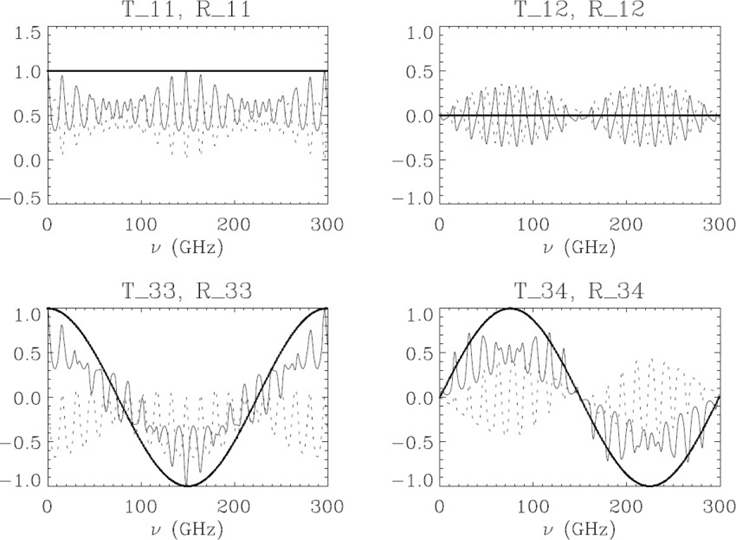
\includegraphics[width=2.5in]{figures/0deg.png}
\caption{Mueller matrix components, for both transmission (T) and reflection (R), of a real Sapphire HWP
optimized for 150 GHz (no ARC). The incoming radiation is at normal incidence \cite{Salatino17}.
}\label{0deg}
\end{figure}

\begin{figure}
\centering
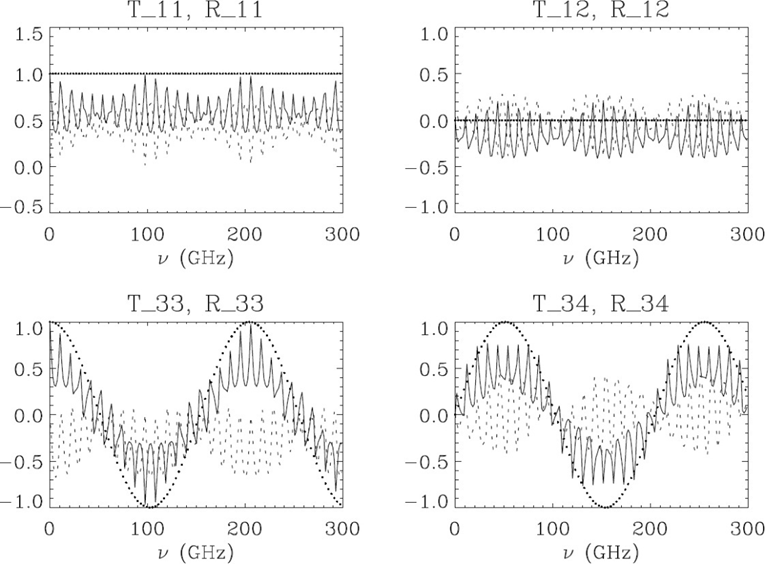
\includegraphics[width=2.5in]{figures/45deg.png}
\caption{Mueller matrix components, for both transmission (T) and reflection (R), of a real Sapphire HWP
optimized for 150 GHz (no ARC). The incoming radiation is at 45deg incidence \cite{Salatino17}.}\label{45deg}
\end{figure}

%------------------------
\subsubsection{Metamaterial HWP}

\begin{figure}
\centering
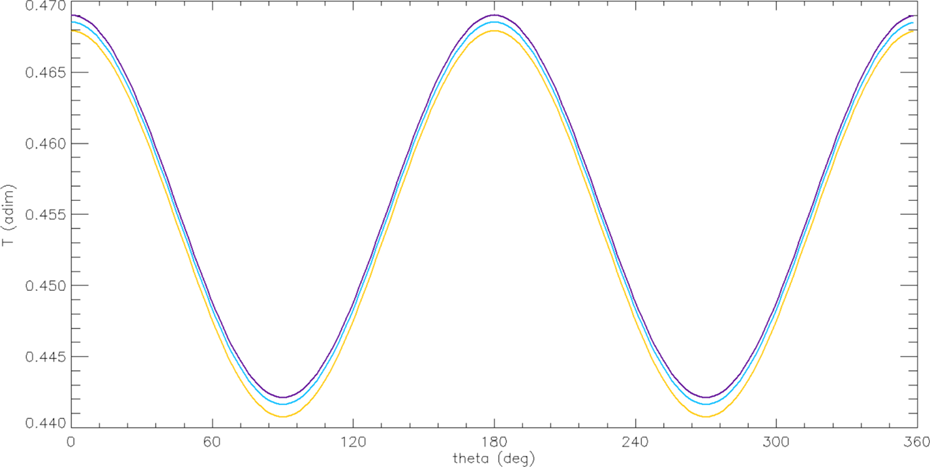
\includegraphics[width=0.6\linewidth]{figures/meta1.png}
\caption{Output signal (dimensionless units) at 70GHz from an unpolarized radiation crossing the AdvACT MF metamaterial HWP. The HWP is %optimized for a frequency band centered
on 90 GHz. Violet line: -10deg, cyan line 0deg and orange 10deg incident angle. At 10deg away from the normal incidence, the output %signal
changes by 0.03.}\label{meta1}
\end{figure}

\begin{figure}
\centering
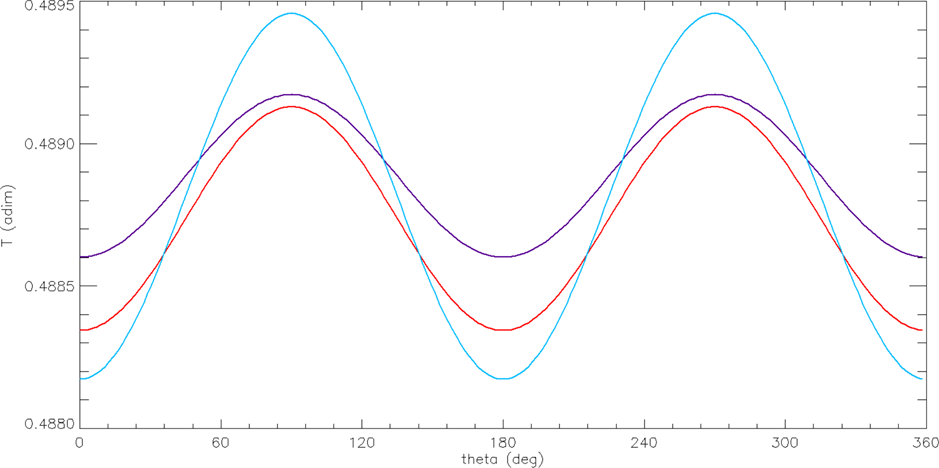
\includegraphics[width=0.6\linewidth]{figures/meta2.png}
\caption{Output signal (dimensionless units) at 90GHz from an unpolarized radiation crossing the AdvACT MF metamaterial HWP. The HWP is %optimized for a frequency band centered
on 90 GHz. Violet line: -10deg, red line 0deg and cyan 10deg incident angle. At 10deg away from the normal incidence, the output signal
changes by 0.0015.}\label{meta2}
\end{figure}

\paragraph{Plan to model and/or measure:}
For a metamaterial HWP, uderstanding of how the optical properties change with the incident angle requires simulations in HFSS or CST. HFSS simulations have demonstrated that the variation in the output signal increases at frequencies closest to the central working frequency of the
HWP (Figs. \ref{meta1} and \ref{meta2}). \textbf{Include these figs.}
Like the birefringent case, FTS and reflectometry measurements can provide experimental estimates of the optical properties.

\textbf{Using the modeled/measured values, how do we model the impact of this response on the science?}

This effect is not modeled in the literature, and could be large in some cases, so the SRF is 4.

\paragraph{Uncertainty/Range:}
\textbf{Add info here as it becomes available.}

\paragraph{Parameterization:}
HFSS/CST simulations can give the optical properties as a function of the incident angle $i$. \textbf{How do we parametrize the science impact}
